%
%===============>>  Симонов Модуль 5 <<=============
%=
\setmodule{5}

%BEGIN_FOLD % ====>>_____ Занятие 1 _____<<====
\begin{class}[number=1]
	\begin{listofex}
		\item занятие 1
	\end{listofex}
\end{class}
%END_FOLD

%BEGIN_FOLD % ====>>_ Домашняя работа 1 _<<====
\begin{homework}[number=1]
	\begin{listofex}
		\item Вычислите: \quad \(\left( \dfrac{36x}{x^2-81}+\dfrac{x-9}{x+9} \right)\cdot\dfrac{x}{x+9}-\dfrac{x}{x-9}\)
		\item Рабочие прокладывают тоннель длиной \( 39 \) метров, ежедневно увеличивая норму прокладки на одно и то же число метров. Известно, что за первый день рабочие проложили \( 4 \) метра туннеля. Определите, сколько метров туннеля проложили рабочие в последний день, если вся работа была выполнена за \( 6 \) дней.
		\item Найдите площадь треугольника, основание которого равно \( 12 \), а высота --- \( 6 \).
		\item Найдите площадь равнобедренной трапеции, меньшее основание которой равно \( 15 \), боковая сторона равна \( 10 \), а высота равна \( 8 \).
	\end{listofex}
\end{homework}
%END_FOLD

%BEGIN_FOLD % ====>>_____ Занятие 2 _____<<====
\begin{class}[number=2]
	\begin{listofex}
		\item Занятие 2
	\end{listofex}
\end{class}
%END_FOLD

%BEGIN_FOLD % ====>>_ Домашняя работа 2 _<<====
\begin{homework}[number=2]
	\begin{listofex}
		\item Решите уравнения:
		\begin{tasks}
			\task \( x^2-x-2=0 \)
			\task \( -x^2+3x-2=0 \)
			\task \( 2x^2-5x+2=0 \)
			\task \( x^2-7x+12=0 \)
			\task \( 0,5x^2-3,5x+6=0 \)
			\task \( x^2-12x+11=0 \)
		\end{tasks}
		\item  Бригада маляров красит забор длиной \(270\) метров, ежедневно увеличивая норму покраски на одно и то же число метров. Известно, что за первый и последний день в сумме бригада покрасила \(90\) метров забора. Определите, сколько дней бригада маляров красила весь забор.
		\item Установите соответствие между графиками функций и формулами, которые их задают.
		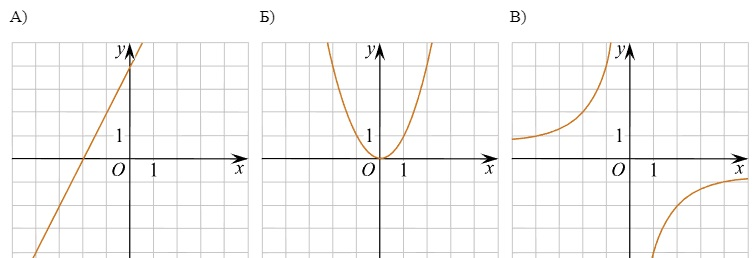
\includegraphics[align=t, width=\linewidth]{/../\picpath/SIMONOVM5H3-1}
		\begin{tasks}
			\task \(y=2x-4\)
			\task \(y=-\dfrac{4}{x}\)
			\task \(y=x^2\)
			\task \(y=2x+4\)
		\end{tasks}
	\end{listofex}
\end{homework}
%END_FOLD

%BEGIN_FOLD % ====>>_____ Занятие 3 _____<<====
\begin{class}[number=3]
	\begin{listofex}
		\item Занятие 3
	\end{listofex}
\end{class}
%END_FOLD

%BEGIN_FOLD % ====>>_ Домашняя работа 3 _<<====
\begin{homework}[number=3]
	\begin{listofex}
		\item ДЗ 3
	\end{listofex}
\end{homework}
%END_FOLD

%BEGIN_FOLD % ====>>_____ Занятие 4 _____<<====
\begin{class}[number=4]
	\begin{listofex}
		\item Занятие 4
	\end{listofex}
\end{class}
%END_FOLD